% Author: Andrew Hughes

\chapter{Algebraic Process Calculi}
\label{apc}

\section{Introduction}

In this chapter, we focus on concurrency from a theoretical
perspective and introduce one of the main algebraic models for
modelling concurrent systems.  The topics and ideas discussed here lay
the foundations for the calculi we will discuss in chapters
\ref{globsync} and \ref{mobility}, and, as a result, are of great
importance in understanding the novel work presented in chapters
\ref{nt}, \ref{dynamite} and \ref{tnt}.

Early computational models took a simple idealised view of the world,
where events occur sequentially and in isolation.  Such a model is the
universal Turing machine \cite{turing:36} which has proven to be
computationally complete; it is capable of simulating all recursive
functions.  However, it does not directly model concurrent execution.

If a model can have this level of computational power without
attempting to represent concurrent behaviour, why is it necessary to
model concurrency at all?  Even though a method of modelling phenomena
exists, and has a certain level of expressivity, it doesn't imply that
it is the most appropriate for a particular context.  The existence of
both Turing machines and the $\lambda$ calculus already demonstrates
this point.  While both have proven equivalent in power, they take
different approaches to achieving this.  However, neither model can
represent the possibility of two or more events occurring at the same
time, and thus can not be used to capture and evaluate the potential
problems which may occur, such as the race conditions illustrated in
the previous chapter.

To see the effect of concurrency on computation, consider a simple
prototypical example, as demonstrated by Milner \cite{milner:lecture}.
Observe the following programs,

\begin{align*}
\mathtt{x} & \mathtt{= 2;}\tag{P1} \\
\\
\mathtt{x} & \mathtt{= 1;}\notag \\
\mathtt{x} & \mathtt{= x + 1;}\tag{P2}
\end{align*}

\noindent where we assume that each line is an atomic
action\footnote{This is a simplification; for example, \texttt{x = x +
    1} actually involves three atomic actions -- reading the value of
  x, computing the value of x plus one and writing the result to x}.

In a sequential system, such as may be modelled by a Turing machine or the
$\lambda$ calculus, both these programs set \texttt{x} to 2.  In such a
system, there is only a single flow of control, so nothing else can
modify the value of \texttt{x}.

However, in a concurrent system, multiple control flows or processes
exist, each running in parallel with the others.  With P1, the value
of \texttt{x} will always be equal to two immediately after execution,
as the assignment takes place within a single atomic action.  However,
in P2, another process is free to modify \texttt{x} (assuming
\texttt{x} is globally accessible) between the assignment of the value
1 and the later summation which makes \texttt{x} equal to 2.

Thus, if P2 is run in parallel with a third program,

\begin{equation}
\mathtt{x = 3;} \tag{P3}
\end{equation}

\noindent then \texttt{x} may end up being either 2, 3 or 4, depending
on whether P3 executes before the first line, after the completion of
P2, or after the first line respectively.  With P1 and P3, only 2 or 3
can result (which one depends on the order the two programs are run).
Again, we have a \emph{race condition}; the final value of \texttt{x}
depends on the timing of the various modifications to its value
performed by the two programs.  As we saw in \ref{semaphores}, the
solution to this problem is to require each program to obtain
exclusive access to \texttt{x} (a lock) for the extent of its use.

This example demonstrates that modelling concurrency is not so much
about multiple programs executing at the same time, but instead
concerns how they may interact.  If each program exists in its own
isolated environment and doesn't access any common resources, then no
interactions will take place and a sequential model for each would be
suitable.  Indeed, this is the way most operating systems handle
running multiple programs.  Thus, it follows that sequential models
are not distinct from concurrent models, but form a subset where this
additional restriction of isolation applies.

The problem is that using sequential models to design and evaluate
programs is becoming more and more detached from the reality of modern
implementations.  For example, many programs now include a graphical
user interface, which must have at least two concurrent threads of
control to be operable; one is needed to await and handle any user
interaction, while the other actually executes the operations of the
program, even if that simply involves updating the display while idle.
As multi-core processors make more machines capable of \emph{true
  concurrency}\footnote{In truly concurrent systems, operations are
  actually performed simultaneously, rather than this being emulated
  by the system scheduler.} and distributed computing paradigms, such
as services, become more prevalent, the need to accurately model the
possible interactions increases.  Concurrency raises issues outside
the reach of traditional sequential models of computation, so to
adequately work with concurrent systems, we need appropriate formal
models to highlight potential flaws and to allow us to account for any
issues that may arise in the design of the program.  Many such models
have been developed, and over the next three chapters, we will
consider a subset of these.

\section{The Calculus of Communicating Systems (CCS)}
\label{ccs}

Algebraic process calculi model the interaction of concurrent
processes using a (usually small) set of algebraic operators, as
opposed to the true concurrency of Mazurkiewicz trace theory
\cite*{maz:trace} or the graphical style associated with Petri nets
\cite*{petri:phd} and Hewitt's Actor model \cite*{hewitt:actor}.
Interaction between processes is via message-passing, rather than via
a common shared memory\footnote{Shared memory and message-passing are
  not orthogonal; a shared memory space may be represented as a
  communicating resource in a message-passing system, while message
  queues can be implemented using shared memory.} or a tuple space
\cite*{linda}.

The foundational calculi in this field are Hoare's CSP
\cite*{hoare:csp78}, Milner's CCS \cite*{milner:ccs} and Bergstra and
Klop's ACP \cite*{acp}, all of which were first developed in the late
1970s to early 1980s.  CSP was originally developed as a programming
language with a relatively large syntax, while Milner aimed for a
minimal calculus.  Both calculi have influenced each other, with CSP
later being refined and given a theoretical basis, following Milner's
work.  ACP shares many of the ideas of CCS, and can be regarded as an
`alternative formulation' \cite{acp}, using a similar set of operators
to achieve a different goal.

In our work, the focus is on CCS, as it forms the basis for most of
the other calculi considered, including the $\pi$ calculus
\cite{milner:pi} (see \ref{picalculus}) and CaSE \cite{CaSE} (see
\ref{case}).  Of the three foundational calculi, CCS has the smallest
syntax with additional features such as failure (represented in both
CSP and ACP) needing to be derived from or appended to this core set.
From a theoretical perspective, this is advantageous, as it makes
reasoning over the calculus simpler, and, as will be seen in later
chapters, further syntax can be added to represent further features if
necessary.

In CCS, processes can be modelled as terms ranged over by $E, F$.
These process terms have the following syntax:

\begin{equation}
\label{ccssyntax}
  E, F\ ::=\ 
  0\ |\ 
  \alpha.E\ |\ 
  E\backslash\ a\ |\ 
  E\ +\ F\ |\ 
  (E\ |\ F)\ |\ 
  X\ |\ 
  \mu X.E\ |\ 
  E[f] 
\end{equation}

\noindent where $\alpha$, $a$ and $f$ are explained below.

External behaviour is described using members of $\names$, an infinite
set of names, and $\overline{\names}$, the corresponding set of
co-names $\{\overline{a} \mid a \in \names\}$.  These names are usually
used to represent \emph{channels} upon which the processes
communicate.  The internal behaviour of the processes is abstracted,
represented simply by the silent action $\tau$.  Under such an
interpretation, $a.E$ (where $a \in \names$) represents a process
whose first action is an input on the channel $a$, whereas
$\overline{a}.E$ (where $\overline{a} \in \overline{\names}$)
represents a process which initially outputs on $a$.  The behaviour of
a process is thus described in terms of atomic actions.  This can be
seen in the first two cases above, where $0$ represents the empty
process (which exhibits no behaviour) and $\alpha.E$ represents action
prefix (used for the limited sequential composition of actions), where
$\alpha \in \actions = \names \cup \overline{\names} \cup \{\tau\}$.

Thus, a basic process is defined as a sequence of inputs, outputs and
silent actions.  Each step in the sequence is a state from which the
process may \emph{perform} an action in order to transition to a new
state.  For example, $a.E$ may perform the action $a$ and become $E$.
We represent this using the notation $a.E \derives{a} E$.

For two processes to communicate with one another, they must
\emph{synchronise}; they must perform a corresponding pair of actions
(e.g. $a$ and $\overline{a}$) at the same time.  For this to occur,
the two processes must be running in parallel.  Parallel composition
in CCS is represented by the $|$ operator.  When two processes are
composed in this way, they may perform their corresponding input and
output actions simultaneously, resulting in a single $\tau$ transition
which changes the state of both processes.

For instance, if $E$ is considered to be $a.E'$ and $F$ to be
$\overline{a}.F'$, then the process formed by the composition of these
two processes, $E|F$ may initially perform one of three actions, $a$,
$\overline{a}$ or $\tau$, to give three possible derivations:

\begin{enumerate}
\item $E\ |\ F \derives{a} E'|F$
\item $E\ |\ F \derives{\overline{a}} E|F'$
\item $E\ |\ F \derives{\tau} E'|F'$
\end{enumerate}

\begin{figure}  
  \centering
\[
\xy
(20,0)*{a.E' \mid \overline{a}.F'}="1";
(0,-15)*{a.E' \mid F'}="2";
(40,-15)*{E' \mid \overline{a}.F'}="3";
(20,-30)*{E' \mid F'}="4";
{\ar@/^2pc/^{a} "1";"3"};
{\ar@/_2pc/_{\overline{a}} "1";"2"};
{\ar@/^2pc/^{\overline{a}} "3";"4"};
{\ar@/_2pc/_{a} "2";"4"};
{\ar^{\tau} "1";"4"};
\endxy
\]
%  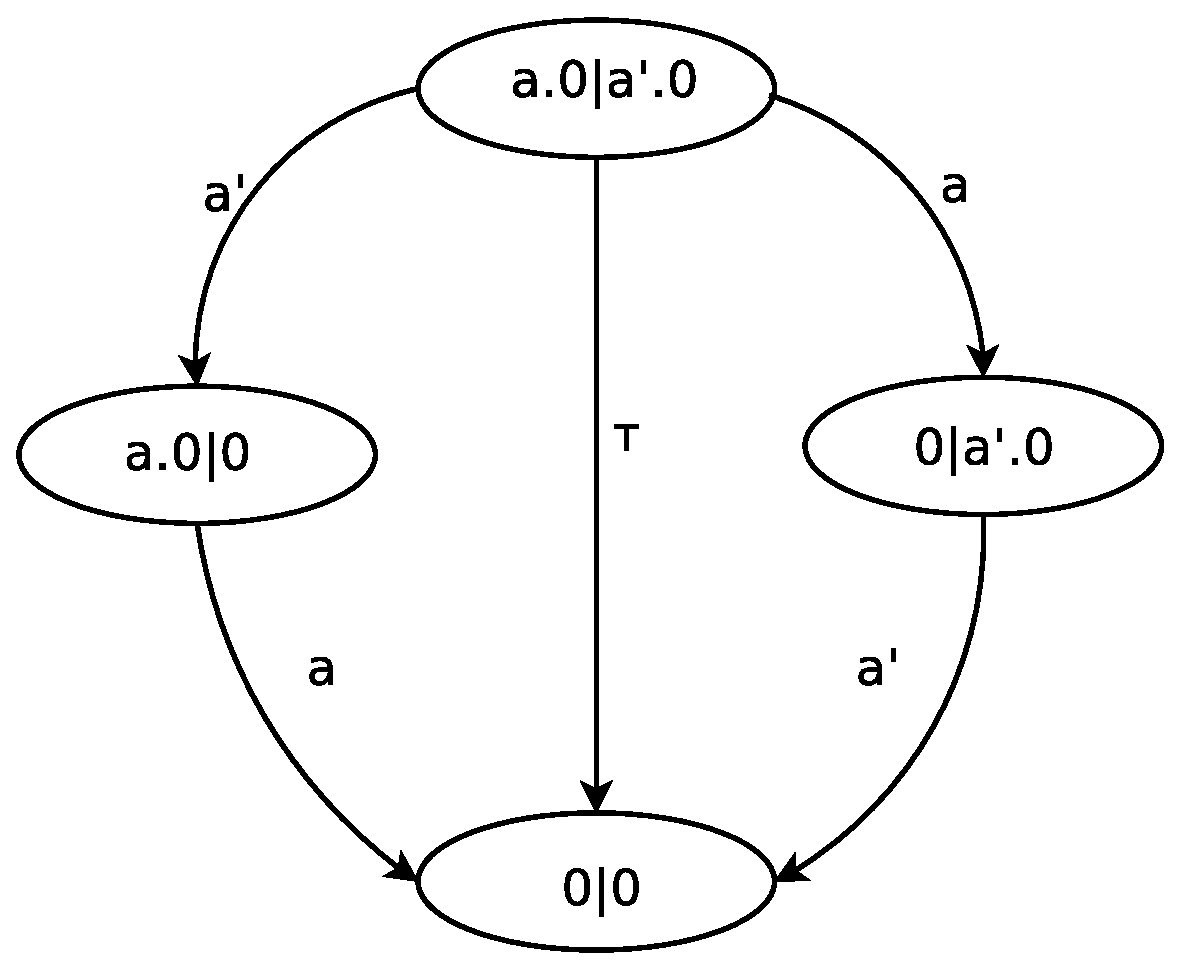
\includegraphics[scale=0.5]{graph1}
  \caption{Graph of $a.0 \mid \overline{a}.0$}
  \label{fig:graph1}
\end{figure}

This is illustrated in Fig. \ref{fig:graph1}.  To make the derivation
of $E|F$ deterministic, the scope of $a$ can be restricted.  In CCS,
an action or co-action can be paired with any complementary action
which is within its scope.  To force the input of $E$ to be paired
with the output of $F$ above, the scope of $a$ must be restricted so
as to include only $E$ and $F$.  This is handled by another operator
in the core syntax, $\backslash$.  Its operand $a$ is the name of a
channel whose scope is restricted to the process given as its left
operand.  So, in this case, $(E|F)\backslash a$ appropriately limits
the possible derivations to just $\derives{\tau}$.

The remaining binary operator is $+$, which provides non-deterministic
choice between two processes.  While the parallel composition operator
represents two processes running in parallel, $+$ corresponds to the
familiar idea of branching found in sequential models.  $E$ and $F$
thus represent two possible behaviours which may or may not occur.
Using the same two exemplar processes again, $E + F$ may derive as
follows:

\begin{enumerate}
\item $E\ +\ F \derives{a} E'$
\item $E\ +\ F \derives{\overline{a}} F'$
\end{enumerate}


\begin{figure}  
  \centering
\[
\xy
(20,0)*{a.E' \mid \overline{a}.F'}="1";
(0,-15)*{F'}="2";
(40,-15)*{E'}="3";
{\ar@/^2pc/^{a} "1";"3"};
{\ar@/_2pc/_{\overline{a}} "1";"2"};
%{\ar@/^2pc/^{\overline{a}} "3";"4"};
%{\ar@/_2pc/_{a} "2";"4"};
%{\ar^{\tau} "1";"4"};
\endxy
\]
%  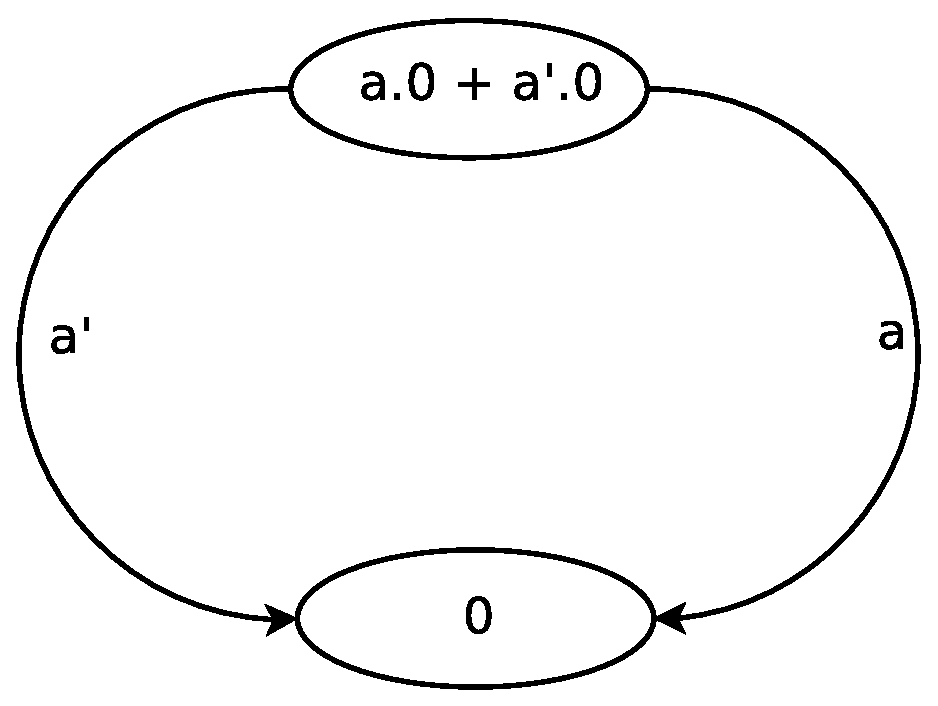
\includegraphics[scale=0.5]{graph2}
  \caption{Graph of $a.0 + \overline{a}.0$}
  \label{fig:graph2}
\end{figure}

Again, this is illustrated in Fig. \ref{fig:graph2}.  There are
clearly similarities between the possible derivations from $E|F$ and
$E+F$, but with choice, there is no possibility of synchronisation and
only one of the two transitions, $a$ and $\overline{a}$ is ever
performed.  The other is lost after the process makes its decision,
whereas with composition, it is possible to perform both actions, one
after the other.

The remaining operators in CCS handle recursion and relabelling.  The
process $\mu X.E$ binds $X$ to $E$, so that later occurrences of $X$
are replaced with $E$.  For example, $\mu X.a.X$ can perform an $a$
transition to become $\mu X.a.X$ again.  The function, $f$, in $E[f]$
has the type $\names \rightarrow \names$ and is used to rename actions
and their complements.  For example, $a.\overline{a}.\tau.0[a
  \rightarrow b]$ is $b.\overline{b}.\tau.0$.

An operational semantics for CCS can be given in terms of a labelled
transition system, $(\procs, \actions, \rightarrow)$, where $\procs$
is the set of CCS expressions formed from the above syntax, $\actions$
is as defined above and $\mathop{\rightarrow} \mathrel{\subseteq}
\procs \times \actions \times \procs$ is the transition relation
defined in Table \ref{tab:ccssemantics}.  We use $E$ and $F$ to range
over process terms ($\procs$), $\alpha$ over the set of actions
($\actions$), $\sigma$ over the set of clocks ($\timers$), $a$ and $b$
over the set of names ($\names$) and and $\gamma$ over $\names \cup
\timers$.

\begin{table}
  \caption{CCS Semantics}
 \label{tab:ccssemantics}
  \shrule
 \vspace{-2mm}
 \begin{center}
 \begin{tabular}{rlrl}
     \Rule{Act}
     {-}
     {\alpha . E \derives{\alpha} E}
     {}
     &
     \hspace{5mm}
     \Rule{Sum1}
     {E \derives{\alpha} E^\prime}
     {E + F \derives{\alpha} E^\prime}
     {}
     \\[3ex]
     \Rule{Sum2}
     {F \derives{\alpha} F^\prime}
     {E + F \derives{\alpha} F^\prime}
     {}
     &
     \hspace{5mm}
     \Rule{Par1}
     {E \derives{\alpha} E^\prime}
     {E \;|\; F \derives{\alpha} E^\prime \;|\; F}
     {}
     \\[3ex]
     \Rule{Par2}
     {F \derives{\alpha} F^\prime}
     {E \;|\; F \derives{\alpha} E \;|\; F^\prime}
     {}
     &
     \hspace{5mm}
      \Rule{Par3}
      {E \derives{a} E^\prime,
        F \derives{\overline{a}} F^\prime}
      {E \;|\; F \derives{\tau} E^\prime \;|\; F^\prime}
      {}
     \\[3ex]
      \Rule{Rec}
      {E \derives{\alpha} E'}
      {\mu X.E \derives{\alpha} E' \{ \mu X.E / X\}}
      {}
      &
     \hspace{5mm}
      \Rule{Res}
      {E \derives{\alpha} E'}
      {E \res{b} \derives{\alpha} E' \res{b}}
      {\alpha \ne b}
      \\[3ex]
      \Rule{Ren1}
      {E \derives{a} E'}
      {E[f] \derives{f(a)} E'[f]}
      {}
      &
     \hspace{5mm}
      \Rule{Ren2}
      {E \derives{\overline{a}} E'}
      {E[f] \derives{\overline{f(a)}} E'[f]}
      {}
 \end{tabular}
  \end{center}
  \shrule
\end{table}

\subsection{The Dining Philosophers}
\label{philosophers}

To fully appreciate CCS, it is necessary to see how it may be used to
model an example scenario.  

Dijkstra's classic `Dining Philosophers' problem
\cite{dijkstra:philosophers} illustrates further issues which may
arise in a situation where multiple processes must interact to achieve
their goal.  In this scenario, five philosophers are seated around a
table, each with a plate of spaghetti and a fork.  The philosophers
divide their time between thinking and eating.  In order to eat, a
philosopher must obtain two forks, necessitating some form of
interaction.  This is a common situation in concurrency, where
multiple parallel processes (the philosophers) need to gain access to
shared resources (the forks).

In cases where things go awry, deadlock or starvation may result.  For
example, if all the philosophers simultaneously pick up the forks on
their left, then none of them will be able to eat; they will all end
up waiting for a fork held by another philosopher.  The system is said
to be \emph{deadlocked}, as none of the processes can obtain a lock on
the resource it needs, as a lock is already held by one of the other
processes\footnote{The solution to breaking this deadlock is to break
  the symmetry; if the fifth philosopher tries to take the fork on the
  right first, he or she will be unable to proceed, but the first
  philosopher will, using the fifth philosopher's left fork.}.
Alternatively, \emph{starvation} may result (literally in this case)
if one of the philosophers never stops eating and consequently never
releases the forks; the resources are unfairly distributed to the
deficit of one of the processes.

Modelling this in CCS involves first ascertaining which processes form
the basis of the system.  Clearly, each philosopher plays a part, so
they should be represented by processes.  Returning to the original
definition of the problem, each philosopher may choose to eat or
think.  In CCS, this can be represented as:

\begin{equation}
Philosopher = Eating + Thinking
\end{equation}

\noindent where the philosopher is recursively defined as making the
choice between $Eating$ or $Thinking$.  Defining the latter is simple;
thinking is simply some internal process of the philosopher:

\begin{equation}
Thinking = \tau .Philosopher
\end{equation}

The focus of the model is on the eating process, which requires access
to the system's shared resources: the forks.  Modelling this
necessitates defining a protocol whereby the philosopher may interact
with the resource in order to obtain access to it.  

\begin{equation}
Eating = \overline{take}.\overline{take}.\tau.\overline{replace}.\overline{replace}.Philosopher
\end{equation}

\noindent which needs to synchronise with two available forks if the
philosopher is to be able to eat (represented by $\tau$) and then
replace the forks again.  It follows that the forks must also be
represented using the process

\begin{equation}
Fork = \mu X.take.Fork^\prime
\end{equation}

\noindent with two communication channels, $take$ and
$replace$.  The fork begins its life on the table from which it
may be \emph{taken}, represented here by the receipt of an input on
the $take$ channel.  Once this has occurred, the process becomes

\begin{equation}
Fork^\prime = replace.X
\end{equation}

\noindent which represents the state where the fork is in use by a
philosopher.  The fork can't be used again until it has received an
input on $replace$, which causes $X$ to be expanded and the fork to
wait for input on $take$ again.

  The system as a whole is modelled by running a number of
  philosophers and forks in parallel, and restricting the scope of the
  fork channels in order to enforce synchronisation.

%\begin{figure}  
%  \centering
%  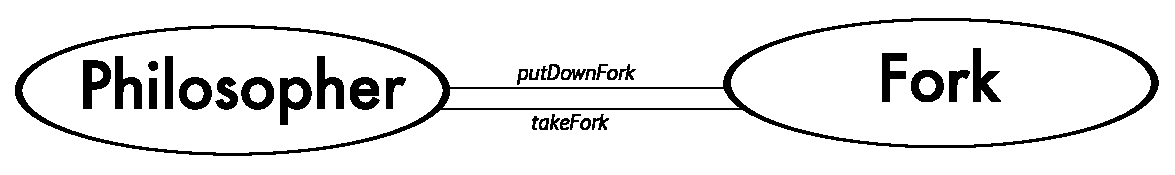
\includegraphics[scale=0.5]{philosophers}
%  \caption{The Dining Philosophers in CCS}
%  \label{fig:dpccs}
%\end{figure}

Note that this CCS representation of the problem only models the
narrative version of the problem above.  There is no attempt to
resolve any of the competition problems, and a strong element of
non-determinism, as to which philosopher gets which fork, still
exists.  It does, however, give a formal representation of the problem
and allows the effects of varying the relative numbers of philosophers
and forks to be observed via simulation.

Modifying this slightly gives a model that corresponds
exactly to a specified number of philosophers and forks, $n$.  From
the definitions above, multiple variants may be generated, such that
each philosopher and fork process has a unique subscript.  For
example, $Philosopher$ becomes $Philosopher_i$, where $i = 1\dots n$.
The same subscripting also applies to the $take$ and $replace$
channels, so that they now correspond to a specific fork.  The
original solution can thus be represented, as the case where each
$Philosopher_i$ initially performs the action $take_i$ (to take
the left fork) and then $take_{i-1}$ (with the exception that when
$i-1 = 0$, we use $n$)\footnote{Again, it is necessary to reverse the
  actions of $Philosopher_n$ in order to obtain a solution that does not
  deadlock.}.

This model restricts which fork is taken by which philosopher
(limiting the possible actions, and thus removing some
non-determinism), but is still prone to questions of non-deterministic
choice (some philosophers may arbitrarily choose to think instead) and
fairness, with regards to action performance (if the actions are
performed in a depth-first manner\footnote{i.e. if an implementation
  always chooses to execute a particular philosopher's choices
  first.}, only one philosopher may end up eating).  These may be
regarded as implementational aspects of the model.

\section{Advantages and Limitations of CCS}
\label{ccslimit}

From its syntax, it is clear that CCS can model sequential behaviour
using sequential composition ($\alpha.E$), non-deterministic choice
($+$) and $\nil$.  This further confirms the intuition noted earlier that
sequential programs are a subset of the larger set of concurrent
programs.  This is illustrated by the $+$ operator, which
returns a smaller set of possible derivations, from the same initial
pair of processes, when compared with parallel composition ($|$).
These sequential operators can also be used to convert a set of
parallel-composed processes into their equivalent interleavings.

CCS can model both sequential and concurrent programs, while still
maintaining a minimal syntax.  A finite axiomatisation can even be
defined, if the simultaneous presence of parallel composition and
recursion is avoided \cite{milner:ccsaxiom}.  However, one fairly
obvious limitation is that there is no data in the model.  The
processes discussed so far don't explicitly communicate anything when
they send or receive signals.  Instead, behaviour arises purely from
synchronisation.  It is possible to extend CCS to represent this by
adding the concept of value passing between processes.  A host of
other process calculi have been based on such a variant of CCS, and we
will consider this in more detail as part of chapter \ref{mobility}.

CCS models are also relatively static; while processes may evolve
(e.g. $a.P$ may become $P$), the communication structure doesn't.
Notably, if a process, $E$, knows about the channels $x$ and $y$
initially, while $F$ only knows about $x$ (due to restriction on $y$),
this status can not change during the course of the various
transitions inherent in the system.  The effect of restriction is more
generally known as \emph{scoping} and occurs frequently with reference
to variables in programming languages.  CCS doesn't allow dynamic
changes to the scoping of channels.  Instead, scoping is fixed to the
static arrangement provided by the initial system, prior to any
transitions.  The addition of dynamic scoping, often referred to as
mobility, is the major contribution of the $\pi$ calculus, a language
based on CCS covered in \ref{scopemobility}.

To conclude, there is another limitation of CCS which is less to do
with a particular concept being absent from the language, instead
being more related to its central aspect: \textbf{synchronisation}.
The problem here lies in the \emph{compositionality} of processes.
While the structure of a CCS system remains compositional, because the
result of parallel composition is determined by the behaviour of the
composed processes together with the rules of the $|$ operator, this
is not true of the synchronisation of arbitrarily many processes.

Consider broadcasting a signal to an arbitrary number of processes.
Ideally, a general \emph{broadcast agent} should be defined which
provides this behaviour.  In CCS, there are at least two ways of
defining semantics for the agent, but not one that provides a suitably
compositional solution.  Perhaps the most obvious is simply to extend
the familiar synchronisation of two processes.  An input and output
pair can synchronise, so why not just create multiple pairs, one for
each receiving process?  For example, transmitting a signal to two
processes can be written simply as

\begin{equation}
\mathbf{\overline{o}.\overline{o}.0} \pc o.P \pc o.Q
\end{equation}

\noindent where the process on the left (in bold) forms the semantics
for the broadcast agent and the processes, $P$ and $Q$, are the
continuations of the input processes

This will work, but what happens when the broadcast agent needs to
transmit the signal to three processes?

\begin{equation}
\mathbf{\overline{o}.\overline{o}.\overline{o}.0} \pc o.P \pc o.Q \pc o.R
\end{equation}

\noindent The semantics of the broadcast agent have to change.  Simply
composing the third input will lead to one of the three being ignored
by the original definition of the broadcaster given above.  So, simply
enumerating multiple synchronisation pairs is not sufficient to
provide a compositional broadcast agent.

A second solution lies in recursion.  If the problem with the previous
solution lies in the broadcasting agent doing too little (i.e. not
transmitting to all the possible receivers), then, by making it
recurse, it will keep sending the output to whoever will synchronise
with it.  Thus, the example for three inputs above becomes

\begin{equation}
\mathbf{\mu X.\overline{o}.X} \pc o.P \pc o.Q \pc o.R
\end{equation}

\noindent which works, and will continue to do so if a further
input process is parallel composed.  

But there is still a problem for much the same reasons as the first
solution.  This works fine on this small scale, but what happens when
this agent is placed in the context of a larger system?  Once the agent
starts its cycle of outputs, it won't stop as there exists
no base case for this recursion\footnote{A base case may be introduced
using non-deterministic choice, but there is no guarantee when this will
be invoked, if ever.}.  An output on $o$ will always be available (within
the scope of any restriction placed on that particular channel) and
the broadcasting process can never do anything else.  The result is a
constantly cycling process, which, in an implementation of this model,
would continue to consume resources.

The true solution to this problem is to enable some form of
\emph{global synchronisation}.  This requires a separate entity,
distinct from the processes involved in the communication, which can
be used to co-ordinate the synchronisation.  In the next chapter, a
branch of process calculi is considered which provides just such a
facility.

\section{Conclusion}

In conclusion, this chapter has taken a brief look at the field of
concurrency modelling, largely from the perspective of process
calculi.  Initially, it was shown that, while universal Turing
machines and the $\lambda$ calculus can simulate any recursive
function, their inherent sequential behaviour makes them unsuitable
for modelling concurrent systems.  CCS, in contrast, can model this
kind of behaviour and in a succinct manner.  However, its minimal
syntax also leads to some limitations.  In the next two chapters, we
will look at some more process calculi, many of which use CCS as their
basis, and observe the benefits of features such as global
synchronisation (see chapter \ref{globsync}) and mobility (see chapter
\ref{mobility}).





